\section{Design}
\label{sec:design}

The architecture of SMON is presented in figure~\ref{xxx}.
The SMON peers run on a set of target machines where
distributed applications will be deployed. Each peer
maintains the full list of target machines as its membership
list. The peers monitor and maintain each other
epidemically. A peer periodically chooses a random neighbour
and sends it a ping message, if the pong message is not
replied within a timeout interval, the neighbour is
considered as failed. The peer will try to recover the
failed peer by restarting it remotely, or deploying and
starting a new peer on fresh machines. Each peer has an
associated version number. The peers exchanges their version
numbers epidemically and peers of lower version upgrade
themselves to the latest versions.

The authentication agent holds the credential (e.g. private
key, password) used to login into the set of target
machines. When a peer wants to restart a failed peer, it has
to first login into the machine of the failed peer. The
authentication agent automates the login process while the
credential is never leaked out.

User uses the client utility to 
app man and extensibility.

\comment{
\subsection{Monitor-reaction model}

%The collective behaviour of all peers defines the runtime
%of a SMON system. 

\begin{figure}
\centering
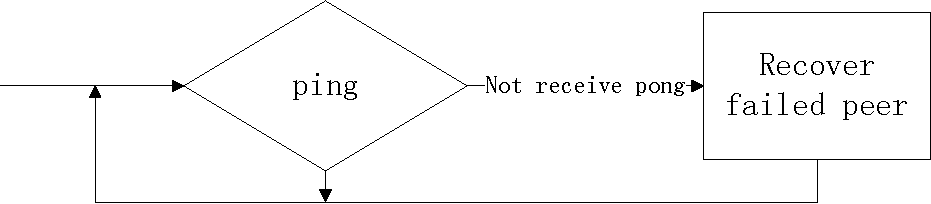
\includegraphics[width=3.0in]{recover}
\caption{recover model}
\label{fig:recover}
\end{figure}

We use a monitor-reaction model to define SMON peer's
behaviours. The model is consistent with and automatically
implements what humans do when maintaining a distributed
system manually. In the model, the ``monitor'' part defines
what status to observe timely, and based on the monitored
result, certain ``reactions'' are performed. Thus, the model
describes a closed-loop control that eliminates human
interventions. For example, a SMON peer will contiually ping
other peers to see if they are running. If a pong message is
not received within a predefined timeout interval, we
consider it as failed and try to recover it by login into
the machine and restart it, otherwise, an empty reaction is
performed. The model is shown in figure~\ref{fig:recover}.

The monitor-reaction model can have varations. First, one
model can be nested in the reaction part of another model.
Using previous example, when we know that a peer is failed,
there can be another reason: the machine is crashed and
maybe replaced by a new one with the same host name. To
handle such cases, in the reaction part we need to further
detect whether the machine has a SMON peer installation, if
not, we have to deploy a copy of the peer first. The model
is shown in figure~\ref{fig:recover-nest}.

Second, two or model models can be combined for purposes
such as optimization. For example, SMON peers also exchange
their version numbers and upgrade peers with low version
automatically. This model can be combined with the failure
detector model by piggyback version number within the ping
message. Thus, we can save one RPC call. The combined model
is shown in figure~\ref{fig:combine}.

One peer may implements several models. They run
concurrently and need to be well coordinated. In the upgrade
model, after a new version is retrieved, the peer need to
start the new verison and stop itself. Before it execute the
action, other models may be running also. The upgrade model
has to wait others until all of them finish actions part.
The coordination can be implemented by using locks, and in
this case, a reader-writer lock may be more suitable.

The models are required to be stateless in the sense that
the execution of a model is independent with it previous
executions. In this way, the implementation of the model is
as simple as possbile and improves peer's reliablity.

\note{transaction? the membership list update should be
atomic.}

\note{the combined model looks complex. the reason: 1. for
optimization. 2. we have carefully examined the code and it
runs for a long time without error?}

The models can not be running infinitely. We address this
problem in subsection~\ref{subsec:livetag}.
}

\subsection{Self-management}

SMON can deploy and maintain itself automatically.

\subsubsection*{Self-deployment}

For a list of target machines, SMON can deploy itself to all
the machines automatically. At the very beginning, there is
not any SMON peer deployed and running yet. At least one
peer must be deployed to a machine and started manually. It
then pings other machines in its membership list and deploys
new peers. The new peers repeat the similar ping-and-deploy
process. While there are more SMON peers deployed and
running, this process speeds up exponentially. It is proved
that with probability 1 all the reachable machines can be
deployed eventually\cite{Eugster2004}.

%The ping-and-deploy process of a SMON peer implements the
%upper part of the ping model in figure~\ref{fig:combine}.
In detail, a peer $P$ periodically choose a random machine
$M$ from its membership list and sends a ping message. If a
pong message is not received within predifined timeout
intervals, it will start the deployment precedure on machine
$M$. $P$ first authenticates itself with $M$ and login into
$M$ automatically (described in in \ref{subsec:security}),
then it copies an installation package of SMON peer to $M$,
starts the package and logout $M$. The installation package
will check the interity of itself (currently using MD5
checksum) in case of transfer errors during copy process.
And it will configure and start the SMON peer.

There may be failures (e.g. connection corrupted, machine
downed) at any time when peer $P$ authenticates and login
into $M$, copies and starts installation package remotely.
When failure happens, $P$ will just abort the deployment
precedure. $M$ will be choosen by another SMON peer at later
time. It is expected that a new SMON peer will be deployed
on $M$ eventually.

Because peers communicate with each other epidemically, it
is possible that two or more peers try to deploy a SMON peer
on the same machine simultaneously. This race-condition is
solved without direct coordination among peers. The
installation packages from different peers will be copied to
different directories and they will not overwrite each
other. The execution of simultaneously started installation
packages are serialized using OS provided sychnization
facilities (currentl lock file). So only the first
installation process will finish and others will abort. In
solving the problem, some overhead is introduced because
multiple installation packages may be copied, which wastes
network bandwidth and storage resources. Through the
evaluation, it is shown that the overhead is low on most
machines. And the size of the installation package is small
(122KB), so the overhead can be considered as insignificant.

It is not easy to define when self-deployment is finished
globally. Ideally, it is finished when all the target
machines are reached and deployed with SMON peers.  However,
considering some machines may be unreachable or shutdown
temporarily, the `finished-globally' situation is rare. Even
after a machine is deployed with SMON peer, it may crash and
replaced with a new machine with the same host name after
some time. The peers then have to continue the
ping-and-deploy process as long as they are live and leave
the `finish' definition to user. The user can query how many
or which peers are deployed, and determine whether it is
appropriate to consider the situation as a finish.

\subsubsection*{Self-upgrade}

As a distributed system, SMON can upgrade itself to a new
version automatically. The upgrade goes online while SMON is
running. User needs not to stop SMON before upgrade.

Each SMON peer has an associated version number and it is
stored persistently in configuration file with the peer.
When two peers communicate using ping-pong messages, they
also piggyback their version numbers in the messages.  If
they find a difference in their versions, the peer with
lower version will retrieve the installation package from
the peer with higher version and upgrade itself
automatically.  It is possbile that a peer of new version is
known by many peers of old version quickly. To avoid flash
crowd, the peer of new version will limit the number of
simultaneous request for retrieving installation package.

To upgrade the whole SMON system to a new version, user only
has to upgrade one peer to the new version and all the other
SMON peers will emerge to the newest versions eventually.
The operator can upgrade a SMON peer by using the client
utility described in subsection~\ref{subsec:client}.


\comment{
\note{need revise the method, consider the ping interval}
When a SMON peer knows there's a new version of peer, a list of
hosts on which peers with new version are running is gathered
through active detection among peers.  A self-upgrade action is
scheduled to read the list and download the new version. At the
beginning of the self-upgrade process, there would only be a
small number of peers running in new version, but they are known
by a lot of other peers.  If there's not any constraints, a lot
of peers may download from the same host simultaneously. To
prevent that, we use a conservative strategy to control the
self-upgrade action.  The destination is, at average, only a
constant $k$ of peers can download simultaneously from a host.
The algorithm we use does not need any coordination among peers,
and works as follows.  If there are $n$ peers want to download
from the same host. Each of them choose to take the download
action  with probability $k/n$. If the action is not taken, it
will be delayed in the next time. So at average, there will be
only $k$ peers downloading from the same host simultaneously,
and it takes a peer to rerun the action $n/k$ times to select
the same peer.  As peers don't coordinate with each other, they
make a conservative estimation that set $n$ to $N$, the number
of all the peers. The strategy may cause a slow start at the
begin of self-upgrade process because $n$ is far smaller that
$N$. When more peers are upgraded to new version, the upgrade
process would be boosted. If a peer knows $p$ peers of new
version, the probability it choose to not download from any of
them is $q=(1-k/n)^p$ and it takes at average $\frac{1}{1-q}$
tries to choose a host. When $p$ increases, $q$ decreases
quickly and $\frac{1}{1-q}$ will be nearly 1 with large $p$.
}

\comment{
It is important to ensure that communication interfaces for
different versions of SMON peers are consistent. If the condition
is ensured, the whole SMON system can be updated gracefully while
most of peers are running and the system functions well.
Otherwise, the new SMON system can only be deployed after the old
one is stopped.
}

\subsubsection*{Self-recovery}

Two kinds of failures may happen and must be handled by
SMON, namely, machine failure and network partition.

Machine failures are handled by self-deployment mechanism.
When a machine fails, the SMON peer running on it is stopped
also.  As soon as the machine recovers, it will be noticed
by some SMON peers quickly and the deployed SMON peer will
be restarted. Starting multiple instances of SMON peer on
the same machine is idempotent to start only one instance
and this is implemented using OS facilities, such as lock
file. When Multiple SMON peer instance is started, the first
one will hold the lock and the others will exit silently.
If the failed machine is replaced with a new one, it will be
installed by a new copy of SMON peer.

Network partitions can also be handled by SMON easily. When
network partition occurs, SMON peers are splitted into
several sub-systems, each of which is connected internally.
Implied by epidemic algorithm, each partitioned part will
eventually converges to the consistent state regarding to
the version of SMON peers. When two partitions rejoin, the
peers in different part will contact and communicate with
each other, leading to the convergence of the whole system.

\subsection{Security}
\label{subsec:security}

SMON peer should be able to login into remote machines
automatically to deploy new peers or restart failed ones.
In this process, the authentication credential should be
keep secret.  \note{here.} It is necessary for different
SMON peers to authenticate each others and keep the
communication confidential among them. In addition, when a
SMON peer deploys new SMON peer on a remote machine, it need
to authenticate itself with the remote machine to copy
contents and execute commands (start the installation
package). The authentication credential is owned by user and
should be protected confidentially. From another point of
view, the SMON peers relies upon the authentication
credentials provided by user to deploy and maintain each
others automatically in a distributed approach. 

SMON system is designed for distributed platforms that are
semi-open---like Planet-Lab or grid, or for proprietary
ones---such as large machine rooms or data centers. It
assumes that: 1) the network between machines in a
distributed infrastructure is not trusted, 2) the users that
can access the infrastructures are not adversarial, 3) the
applications running in the infrastructures are not
adversarial. Based on assumptions above, SMON designed an
security mechanism which guarantees that 1) communications
among SMON peers are authenticated and confidential, 2)
authentication credentials are never leaked. The mechanism
incorporated in current design supports challenge based
authentications like public-key authentication scheme, which
is extensively used.

To achieve that goal, SMON includes an separate
authentication agent acting as the authentication bootstrap
for SMON.  Whenever a SMON peer needs to login into a
machine, it will indirect the authentication challenges to
the agent and the agent will solve the challenges and send
the result back. In this way, the authentication credentials
are kept secret for all the times. A symmetric encryption
key $K_E$ is shared among all the SMON peers and the
authentication agent. It is used to authenticate peers and
agent within the same SMON system, and establish
confidential communication channels among them. The shared
key $K_E$ is included within the installation package of the
SMON peer. When a SMON peer is deployed, $K_E$ is deployed
along. Note that $K_E$ is never leaked out of network during
deployment. $K_E$ is safe to be stored within local machines
based on assumption 2) and 3), and further local security
mechanisms can be leveraged to protect $K_E$, such as file
system read/write permissions.

\comment{
It is not necessary to keep authentication agent running for
all the time.  When the self-deployment process is finished,
the agent can be closed, and re-open timely for maintennace
purpose.  It is also a security concern to offline
authentication agent to protect user authentication
credentials.
}

The authenticate agent can be also replicated if required.
When a SMON system is deployed at large enough scales, there
can be multiple instances of authenticate agent for
performance considerations. Name server based load balance
mechanism\cite{} can be used to direct SMON peers to their
nearest agents.

\subsection{Membership}

The membership maintenance of SMON system is different from
other distributed systems. While other distributed systems
maintains a list of peers that are currently running, SMON
maintains a list machines on which there should be peers
running.  And an important requirement of SMON is, even when
there is only one SMON peer running, it should be able to
know all the target machines that SMON need to be deployed.
The implication is that every running SMON peer should be
able to know the full list of target machines.

In current design, a simple scheme is used that each SMON
peer will store a replica of the full list of target
machines persistently in compressed format. The list also
has an associated version number. User can update the
membership list to change the set of machines on which SMON
runs.
%To reduce the communication overhead in updating membershit
%list, only the differences between two version are
%propagated during machine list update process. 
This scheme is enough for handling machine list containing
even tens of thousands of machines because only the machine
names or IPs are stored in the list.  An estimation shows
that, storing 15000+ machines names in zip format takes
about 100K bytes, which is an acceptable result.

When membership changes, newly add machines will be deployed
with new SMON peers. The peer running on removed machines
will receive the new machine list and find that they are not
in the list. It will stop all the models \note{here} and
just replies to incoming monitor messages. In this way, it
helps spreading membership changes. After most peers update
their member list, the peers in removed machines will kill
themselves after they haven't received any messages for
enough long time.

\note{below here are not checked.}

\subsection{Control the running of the model}
\label{subsec:livetag}

Without any control, a monitor-reaction model can be running
forever and this may cause problems. For example, when we
want to stop a distributed application, we first stop
application processes on each machine and then try to stop
the SMON system. But the uncontrolled self-management model
makes SMON unstoppable. If we stop any SMON peer on a
machine, it will be started soon by another peer. The only
solution under such conditions is to stop all the SMON peers
simultaneously, which is not feasible at large scale.

We use a boolean variable called livetag to control
monitor-reaction models. Before running of a model, the
value of the livetag is checked, if the value is false, the
model will not be executed. To stop a SMON system, we can
set the livetag to false and all peers stop running
implemented models. We can stop SMON peers one by one now.

The livetag variable has an associated version number and is
maintained on each peer using a separate monitor-reaction
model. The peers exchanges <livetag, version> tuples and
update the tuple to latest version. Even the livetag model
is controlled by the value of livetag. When livetag is
false, peers stop running any models but still responds to
incoming messages, so as to help disseminating the update to
livetag.

\comment{
The SMON system has a global state indicating it is active
or not. When SMON is active, the peer-monitoring component
is enabled. Every SMON peers actively monitor each others
and keep them running as possible as they can. While SMON is
not active, the peer-monitoring function is disable and SMON
acts just like an usual management tools. The active state
is an essential part of SMON system design. Without it, SMON
is just another usual management tool for distributed
applications. If the state is designed as active all the
time, it is a hard problem to stop an active SMON system. If
we try to stop the SMON peers one-by-one, we will noticed
that the stopped peers will soon be restarted by other
peers. And the only way to stop an active SMON system is to
stop all the peers near simultaneously, which is quite hard.
The active state also has an associated version number and
each SMON peer replicates and stores the state with version
locally.  The epidemic algorithm is used to maintain the
state consistently and efficiently among all peers.
}

\subsection{Application management}

One or more distributed applications can be managed by SMON.
Each SMON peer manages the application peers that run in the
same machine. SMON peers knows the existence of a new
application through periodically communicating with each
other. For each application, an instance of application
manager model is started.  A new application entry is
created if it is known for the first time.  The peers
download the application with specified version from other
peers. There is a set of implemented RPC calls for control
and monitoring of managed applications.

%Each of the managed application peers has an
%associated version number.  The version numbers of
%application peers are maintained by managing SMON peers. The
%similar epidemic algorithm is used for keeping application
%peers up-to-date. A trick used in application management is,
%when an application peer has not been deployed on a machine
%yet, its version number is set to 0.0, which is smaller than
%any real version numbers. In this way, application
%deployment problem is turned to the application update
%problem.

The application installation package should contain a
configuration file. The file specifies which binary file to
start when the application is installed, if the application
process failed, what actions to perform. The choices may be
no action, restarting the application for $N$ times, or
reporting the failure event.

\subsection{Client utility}
\label{subsec:client}

A client utility is provided for user to control and query
the system and query the system on demand. With the utility,
user can install or update SMON, install a new application,
or query SMON and applications' status.

\comment{
SMON, live? version?

query app, live?

update version

install application

set/query livetag, 

maintain version number of SMON and live tag
}

To improve reliability, the one-hop source
routing\cite{Gummadi2004} algorithm is implemented. When the
utility failed to communicate directly with a peer, it
randomly selected $k$ ($k=4$ in current design) other peers
for redirecting the message.  This feature is useful for
managing large number of machines. We implement this mechanism
because we notice a lot of connection problems caused by
name resolution error. It happens between our laptop and
PlanetLab machines, and also among some PlanetLab machines.  In
the experiment, we noticed a machine cannot connect to other
two machines because of name resolution error for more than one
day.  But through one-hop source routing, they can
communicate without problem. This feature is useful for
users to control or monitor machines at large scale. As the
user control or monitor other machines through a peer as proxy,
one-hop source routing can increase the number of connected
peers.

% vim:foldmethod=marker:textwidth=60
